\section{Detaillierte Berechnungen}
\label{anhang-Berechnungen}
Damit wir wissen, mit welchen Geschwindigkeiten wir die Bälle abwerfen müssen, haben Berechnungen gemacht.
Hier sind nur die Hauptergebnisse angezeigt; alle Berechnungen befinden sich \href{https://github.com/accefa/doku/tree/master/bin/Berechnungen.xlsx}{hier}. \\ \\
Mit der Benutzung und der Anwendung der schrägen Wurf Formel, könnten wir die nötige Geschwindigkeit ausrechnen und damit die notwendige Energie.
\begin{figure}[h!]
	\centering
	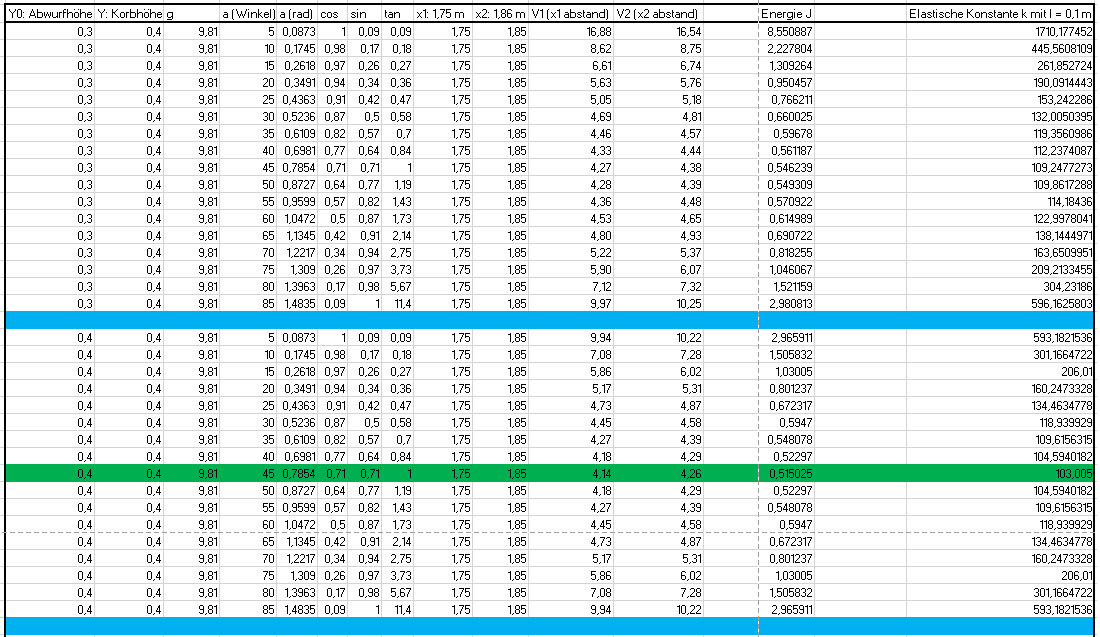
\includegraphics[width=1\textwidth]{../../fig/Geschwindigkeit_und_eleastische_Konstante.png}
	\caption{Berechnungen der Benötigten Abwurfgeschwindigkeiten und der nötigen Federkonstante}
	\label{fig:Berechnungen von die Geschwindigkeit}
\end{figure}
\newpage
Um eine Idee von den nötige Drehmomenten, die unseres Motor braucht, wurden die benötigten Trägheitsmomenten berechnet. Anhand der Trägheitsmomente konnte die Leistungen und die Drehzahlen berechnet werden.
\begin{figure}[h!]
	\centering
	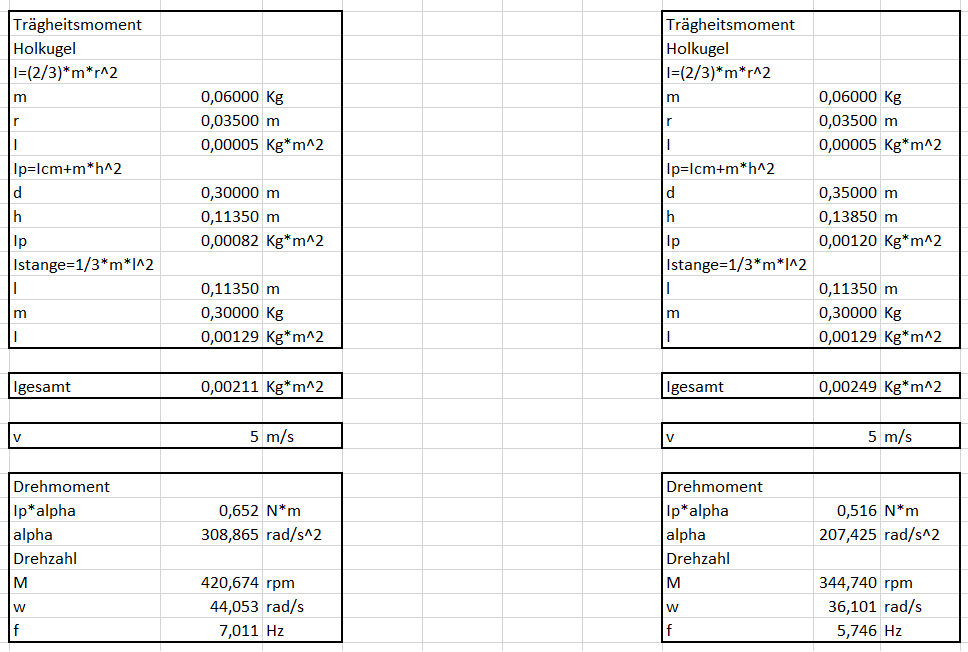
\includegraphics[width=1\textwidth]{../../fig/Berechnungen_Propeller.png}
	\caption{Notwendige Drehzahlen und Drehmomente vom Motor für das Konzept Propeller}
	\label{fig:Berechnungen für der Propellerkonzept}
\end{figure}

Die genauen Berechnungen sind auch im Berechnungsfile auf GitHub zu finden. 